\chapter{APPLICATIONS OF PLASMA-LIQUID SYSTEMS}
\label{chap:applications}

\section{Fertigation}
\label{sec:fertigation}

For a published version of much of the fertigation work described below, the author encourages the interested reader to navigate to \cite{Lindsay2014}.

\subsection{Experiment}

\subsubsection{PAW for Plant Treatment}

The glow discharge is generated using a single-stub matched coaxial structure and a 162 MHz power source.  For detailed design and electrical characteristics, see \cite{byrns2012vhf}.   Delivered power to the plasma was held constant at 420 W; the air feed gas was flowed at .11 m3/min.  To generate a single "batch" of PAW, 1.9 L of distilled water was exposed to the air discharge for 72-80 minutes.  The height of the treatment container was controlled such that the discharge was held roughly .5 cm above the water surface for the duration of exposure.  Treatment time was chosen such that the final water pH was 2.7.  PAW batches were stored at acidic pH for two days and then NaHCO3 was added until a plant friendly pH of 6 was achieved. Final nitrate and nitrite concentrations were determined using ion chromatography (IC), and were between 113-120 ppm and 4-6 ppm respectively. A new batch of PAW was created once every two days in order to keep up with plant watering demand.  A representative experimental set-up for exposure of water to the glow discharge can be seen in \cref{fig:batch_scheme}.

\begin{figure}[htbp]
  \centering
  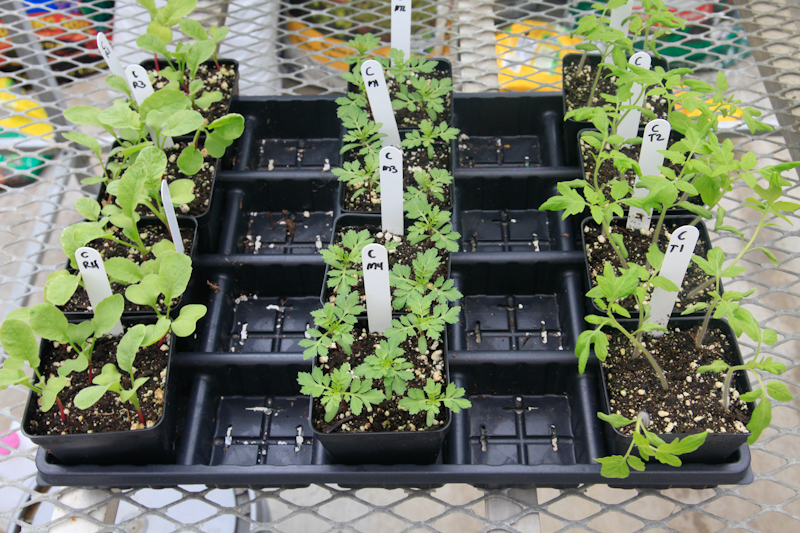
\includegraphics[width=0.9\textwidth]{Figure2_word.jpg}
  \caption{CC group potting arrangement during weeks 1 and 2 (germination phase).  Photo taken at end of week 2. For scale, each pot is 8.9 cm x 8.9 cm x 6.1 cm (length x width x height)}
  \label{fig:cc}
\end{figure}

\begin{figure}[htbp]
  \centering
  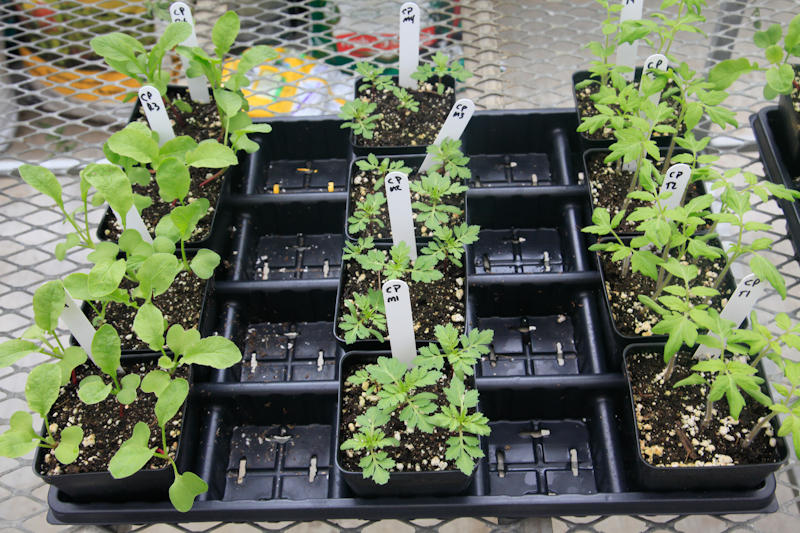
\includegraphics[width=0.9\textwidth]{Figure3_word.jpg}
  \caption{CP group potting arrangement during weeks 1 and 2 (germination phase). Photo taken at end of week 2. For scale, each pot is 8.9 cm x 8.9 cm x 6.1 cm (length x width x height)}
  \label{fig:cp}
\end{figure}

\begin{figure}[htbp]
  \centering
  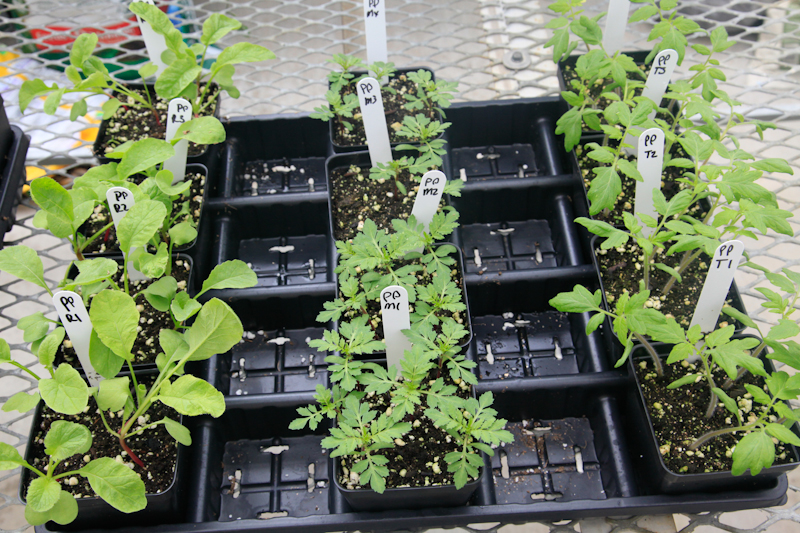
\includegraphics[width=0.9\textwidth]{Figure4_word.jpg}
  \caption{PP group potting arrangement during weeks 1 and 2 (germination phase). Photo taken at end of week 2. For scale, each pot is 8.9 cm x 8.9 cm x 6.1 cm (length x width x height)}
  \label{fig:pp}
\end{figure}

In a four week fertilizer experiment, Janie marigolds, Better Boy tomatoes, and Early Scarlet radishes were subjected to three different treatment types.  A control-control (CC) group was given control water (tap water) for the four-week duration.  A control-plasma (CP) group received control water for two weeks and then PAW for weeks 3 and 4; a plasma-plasma (PP) group received PAW throughout.  During the germination phase, weeks 1 and 2 of treatment, the plants were arranged as shown in \cref{fig:cc,fig:cp,fig:pp}.  Plant potting soil was composed of 60\% Canadian sphagnum peat, 20\% horticultural grade vermiculite, and 20\% horticultural grade perlite; all ingredients were blended together and brought to a moisture content of 50\% before potting.  A standard greenhouse environment was used with temperatures between 24 and 29 degrees Celsius during the day and between 16 and 21 degrees Celsius at night.  Additional experiments not discussed here indicate too much sunlight may negatively affect plant growth irrespective of water treatment type; consequently, shade curtains were used in the presented study to mitigate that effect.

At the end of the germination phase, a representative plant from each pot was chosen for treatment during the growth phase, weeks 3 and 4.  All other plants were removed from the pot.  This is exemplified by \cref{fig:cp_growth}.

\begin{figure}[htbp]
  \centering
  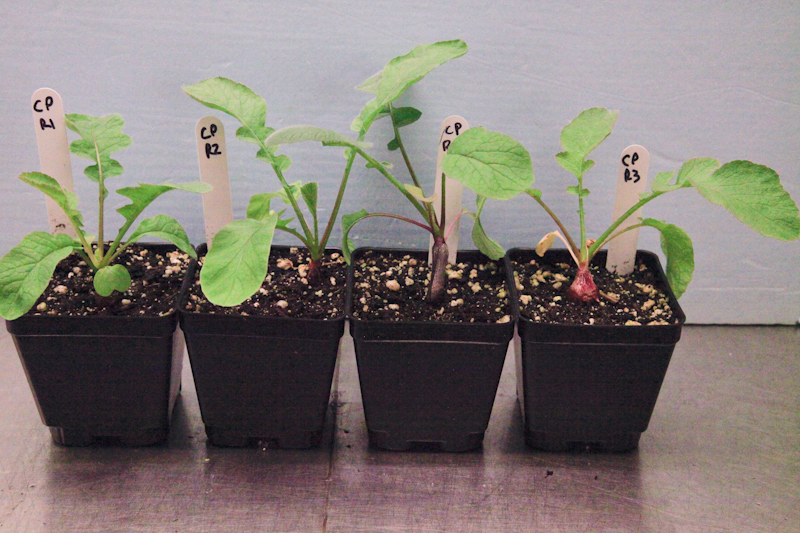
\includegraphics[width=0.9\textwidth]{Figure5_word.jpg}
  \caption{Potting arrangement during weeks 3 and 4 (growth phase) for CP group radishes.  A single representative plant from each pot was chosen at the end of the germination phase to continue on during the growth phase. For scale, each pot is 8.9 cm x 8.9 cm x 6.1 cm (length x width x height). Note that the 8.9 cm x 8.9 cm dimensions refer to the pot’s top as opposed to its base}
  \label{fig:cp_growth}
\end{figure}

During the germination phase, plants were misted 4-5 times per day; during the growth phase, plants received a traditional garden-style watering, e.g. steady water stream, 1-2 times per day.

\subsubsection{Dependence of nitrogen species concentrations on system variables}

After performing the fertilizer experiment, additional research has focused on optimizing and understanding generation of nitrates and nitrites in aqueous solution.  Several variables have been explored, including power supplied by the 162 MHz generator, flow rate of the feed gas, type of interface between the plasma and water phases, and the effect of aqueous impurities, particularly basic species.  Power was regulated to provide constant delivered power to the load.  It was controlled using a remote interface and was varied in these experiments between 385 and 700 Watts delivered power.  Reflected power ranged from 5 to 100 W and was dissipated into a 50 Ω circulator at the generator output.  Gas flow rate was measured using a .57 m3/min maximum capacity in-line flow meter and was varied between .085 and .42 m3/min.  The third variable investigated was the type of interface between plasma and water phases.  The majority of experiments were performed using the experimental set-up shown in \cref{fig:batch_scheme}.  However, in a preliminary investigation of increasing the surface area of interaction between the two phases, a green-house sprayer was used to directly inject water droplets from the side of the device, through the active plasma region, and into a collecting beaker on the other side; an illustration of the set-up is shown in \cref{fig:spray_scheme}.  The number of impurities and basic species in water is controlled in two manners.  The first is the choice between distilled and tap water, with the former containing negligible impurities and the latter containing impurities found in Raleigh's municipal water supply; these impurities are summarized in \cref{tab:tap_water}.  The most relevant item in \cref{tab:tap_water} is the alkalinity, which comes primarily from the carbonate system.  At a pH of 8.4, it is reasonable to assume that the tap water alkalinity is completely due to bicarbonate. \cite{benjamin2014water} Using this assumption, the concentration of bicarbonate in tap water is .50 mmol/L.  The concentration of bicarbonate can also be directly controlled by adding measured amounts of NaHCO3.   NaHCO3 can be added pre- or post-exposure depending on the experiment.  The motivation for adding basic species like NaHCO3 to solution is that they are known to react with dissolved NO and NO2 to form nitrite. \cite{greenwood1984chemistry} Thus basic species concentrations can be a control knob for adjusting the nitrogen chemistry in PAW.

\begin{table}[htpb]
  \begin{center}
    \begin{tabular}{|c |c |}
      \hline
      pH & 8.4 \\\hline
      Free CO$_2$ & .23 \\\hline
      Total alkalinity (mg/L as CaCO$_3$) & 24.8 \\\hline
      Total hardness (mg/L as CaCO$_3$) & 24.4 \\\hline
      Total dissolved solids (mg/L) & 150 \\\hline
      Specific conductivity ($\mu$S/cm) & 225 \\\hline
      Iron (mg/L) & .01 \\\hline
      Manganese (mg/L) & .02 \\\hline
      Fluoride (mg/L) & .78 \\\hline
      Chloride (mg/L) & 13.3 \\\hline
      Silica (mg/L) & 8.12 \\\hline
      Silt density index (SDI) & 5.00 \\
      \hline
    \end{tabular}
  \end{center}
  \caption{Impurities in Raleigh tap water}
  \label{tab:tap_water}
\end{table}

\subsection{Results}

\subsubsection{PAW for plant treatment}

As explained in the experimental section, at the end of two weeks, a representative plant from each pot was chosen to continue into the growth phase.  At that time the height of the representative plants was recorded; this resulted in a sample size of eight plants for each control strain (radish, marigold, and tomato) and a sample size of four plants for each plasma strain (radish, marigold, and tomato).  The control sample size was twice as large as the plasma sample size because both CC and CP groups received tap water through the first two weeks.  The average height of these plants is shown in \cref{fig:germ_heights}. PAW treated plants showed a larger average height than their control treated counterparts; however, a two-tail Welch's t-test showed that none of the differences were statistically significant for a significance level of .05.  The t-test results are summarized in \cref{tab:germ_heights_t}.    The number of sprouted seedlings per pot was also counted and is presented in \cref{fig:germ_sprouts}.  Though the number of sprouted seedlings per pot was higher for control radishes and tomatoes compared to plasma groups, the differences were not statistically significant as indicated again by a two-tail Welch's t-test with a significance level of .05.  The t-test results for the number of sprouted plants per pot are summarized in \cref{tab:germ_sprouts_t}.

\begin{figure}[htbp]
  \centering
  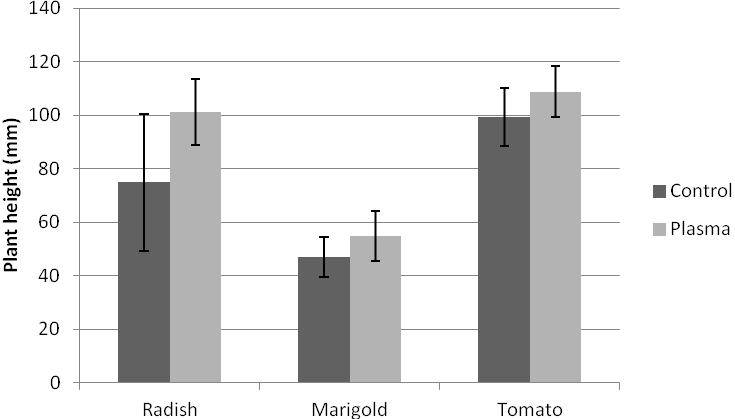
\includegraphics{Figure7_word.png}
  \caption{Comparison of control and plasma treated plant heights at end of germination phase (end of week 2) with accompanying error bars}
  \label{fig:germ_heights}
\end{figure}

\begin{table}[htpb]
  \begin{center}
    \begin{tabular}{c |c |c }
      Radish & Marigold & Tomato \\
      \hline
      .054 & .243 & .219
    \end{tabular}
  \end{center}
  \caption{Two-tail Welch's t-test results comparing control and plasma treated plants at end of germination phase.  Values shown are p-values}
  \label{tab:germ_heights_t}
\end{table}

\begin{figure}[htbp]
  \centering
  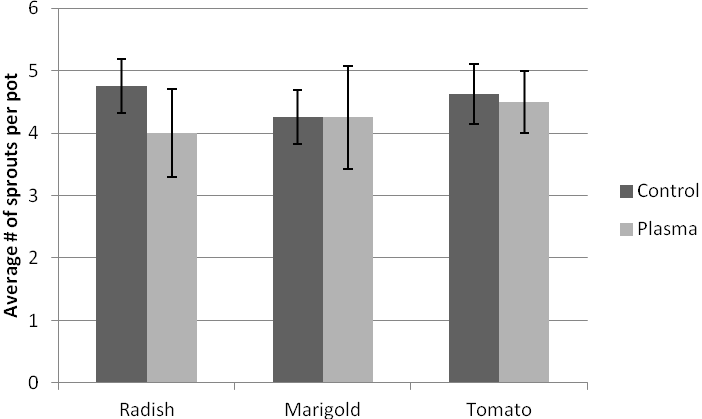
\includegraphics{Figure8_word.png}
  \caption{Comparison of control and plasma treated sprout data at end of germination phase (end of week 2) with accompanying error bars}
  \label{fig:germ_sprouts}
\end{figure}

\begin{table}[htpb]
  \begin{center}
    \begin{tabular}{c |c |c }
      Radish & Marigold & Tomato \\
      \hline
      .163 & 1 & .728
    \end{tabular}
  \end{center}
  \caption{Two-tail Welch's t-test results comparing the number of sprouted plants per pot for control and plasma treated plants at end of germination phase.  Values shown are p-values}
  \label{tab:germ_sprouts_t}
\end{table}

Beginning at the start of the growth phase, plant dimensions were measured almost daily. Because of practical difficulties with measuring the height, the distance spanned by the plants' true leaves was recorded.  Measurements are plotted in \cref{fig:radish_span,fig:marigold_span,fig:tomato_span}. Plants receiving PAW during this phase of the experiment, e.g. CP and PP groups, showed a marked improvement in growth relative to the CC group.

\begin{figure}[htbp]
  \centering
  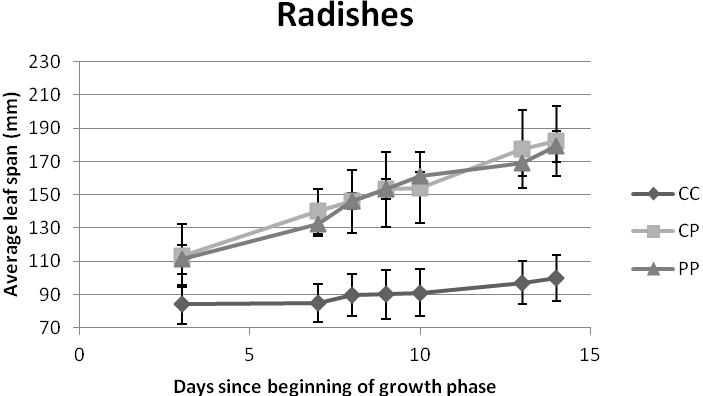
\includegraphics{Figure9_word.png}
  \caption{Average radish leaf span vs. time (growth phase, weeks 3 \& 4)}
  \label{fig:radish_span}
\end{figure}

\begin{figure}[htbp]
  \centering
  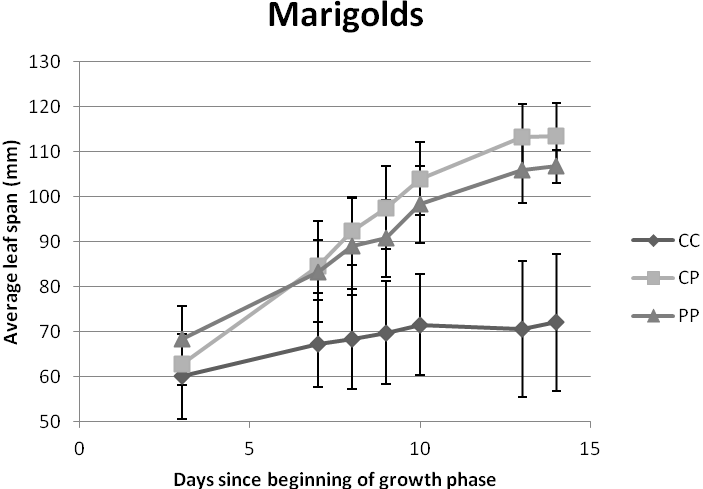
\includegraphics{Figure10_word.png}
  \caption{Average marigold leaf span vs. time (growth phase, weeks 3 \& 4)}
  \label{fig:marigold_span}
\end{figure}

\begin{figure}[htbp]
  \centering
  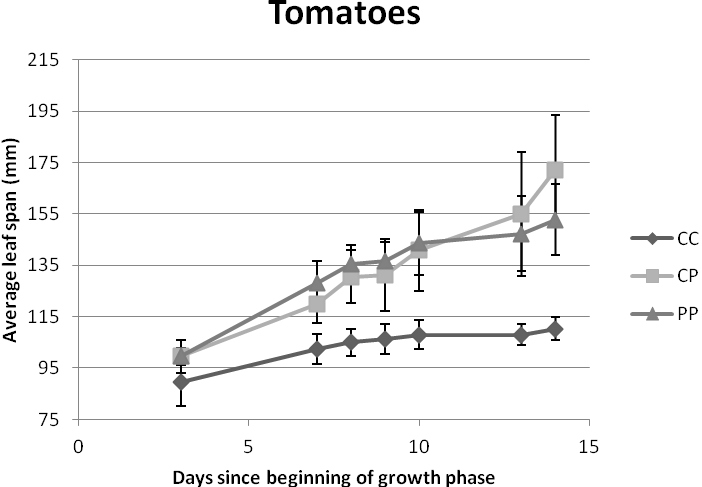
\includegraphics{Figure11_word.png}
  \caption{Average tomato leaf span vs. time (growth phase, weeks 3 \& 4)}
  \label{fig:tomato_span}
\end{figure}

In addition to the leaf span measurements recorded throughout the growth phase, photographs of representative plants were taken at the end of experiment in order to visually compare the relative sizes of the CC, CP, and PP groups.  These photos are shown in \cref{fig:radish_pic,fig:mari_pic,fig:tomato_pic}. CP and PP plants were larger in size than their CC counterparts.

\begin{figure}[htbp]
  \centering
  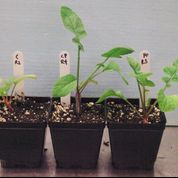
\includegraphics{Figure12_word.jpg}
  \caption{Representative radish plants at end of experiment. Left pot is CC; center is CP; right is PP}
  \label{fig:radish_pic}
\end{figure}

\begin{figure}[htbp]
  \centering
  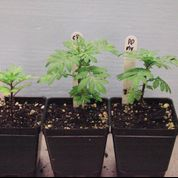
\includegraphics{Figure13_word.jpg}
  \caption{Representative marigold plants at end of experiment. Left pot is CC; center is CP; right is PP}
  \label{fig:mari_pic}
\end{figure}

\begin{figure}[htbp]
  \centering
  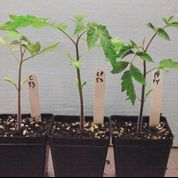
\includegraphics{Figure14_word.jpg}
  \caption{Representative tomato plants at end of experiment. Left pot is CC; center is CP; right is PP}
  \label{fig:tomato_pic}
\end{figure}

After the above photos were taken, plants were removed from their pots, washed, and dried.  Roots were separated from the above-ground plant called the shoot and both sections were weighed.  Average shoot and root dry weights are summarized in \cref{fig:shoots,fig:roots} respectively.  In agreement with \cref{fig:radish_pic,fig:mari_pic,fig:tomato_pic}, the average shoot masses of CP and PP plants were larger than CC plants.  A t-test, summarized in \cref{tab:shoot_t}, showed that all of these differences were statistically significant except for the difference between PP and CC marigolds (however, its test statistic of .06 was very close to our significance cut-off of .05).  In marigolds and tomatoes CP shoot masses were greater than PP shoots, however, the differences were within the error of the measurement.  Root mass results did not track with the shoot sizes and masses.  The root masses of CC radishes were on average larger than CP and PP radishes. CP marigold and tomato root masses were greater than their PP counterparts which were in turn larger than CC root masses.  However, all of the root mass differences were within the error of the measurement, and the t-test summarized in \cref{tab:root_t} indicates that the differences are not statistically significant.

\begin{figure}[htbp]
  \centering
  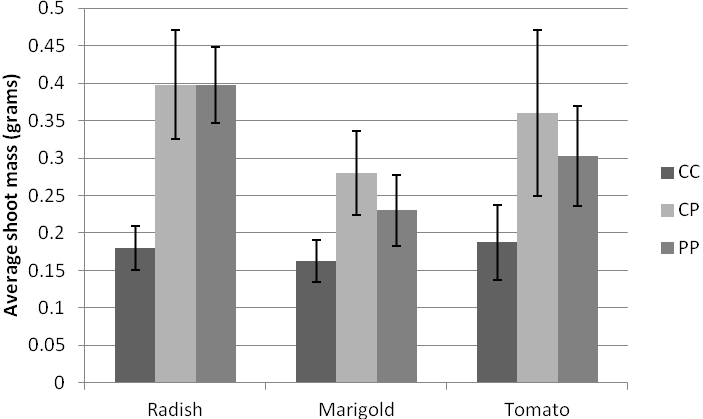
\includegraphics{Figure15_word.png}
  \caption{Average shoot dry mass by plant and treatment types at end of experiment}
  \label{fig:shoots}
\end{figure}

\begin{figure}[htbp]
  \centering
  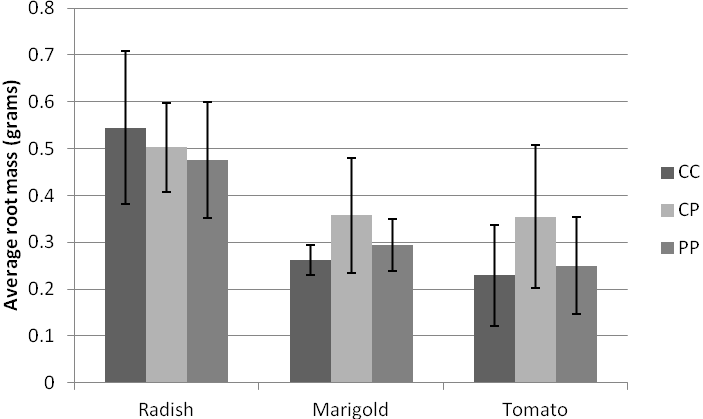
\includegraphics{Figure16_word.png}
  \caption{Average root dry mass by plant and treatment types at end of experiment}
  \label{fig:roots}
\end{figure}

\begin{table}[htpb]
  \begin{center}
    \begin{tabular}{|l |c |c |c |}
      \hline
      Shoot Mass & PP vs. CP & PP vs. CC & CP vs. CC \\\hline
      Radish & 1.000 & 0.001 & 0.005 \\\hline
      Marigold & 0.224 & 0.060 & 0.017 \\\hline
      Tomato & 0.414 & 0.035 & 0.044 \\\hline
    \end{tabular}
  \end{center}
  \caption{p-values for comparisons between the shoot masses of different plans and treatment groups. Values below .05 indicate a statistically significant difference between the species being compared}
  \label{tab:shoot_t}
\end{table}

\begin{table}[htpb]
  \begin{center}
    \begin{tabular}{|l |c |c |c |}
      \hline
      Root Mass & PP vs. CP & PP vs. CC & CP vs. CC \\\hline
      Radish & 0.738 & 0.523 & 0.674 \\\hline
      Marigold & 0.402 & 0.360 & 0.218 \\\hline
      Tomato & 0.304 & 0.798 & 0.235 \\\hline
    \end{tabular}
  \end{center}
  \caption{p-values for comparisons between the root masses of different plans and treatment groups. Values below .05 indicate a statistically significant difference between the species being compared}
  \label{tab:root_t}
\end{table}

\subsubsection{Dependence of nitrogen species concentrations on system variables}

Following the plant experiment, focus shifted to understanding and optimizing the generation of nitrate in solution.  The first variables explored were input power and energy delivered to the plasma.  At a gas flow rate of .14 m3/min, an exposure time of 3 minutes, and a treatment volume of 150 mL distilled water, nitrate concentrations were determined for powers ranging from 385 to 630 W and are shown in \cref{fig:nitrogen_vs_energy}.  For a better comparison with spray treatment results shown in \cref{fig:nitrogen_vs_energy_spray}, the horizontal axis is defined in terms of the energy deposited in the plasma per mass of water exposed to the plasma.  The results indicate a general downward trend in nitrate concentration with respect to power and total energy deposition.   To decouple the effects of power and total energy deposition, a second experiment was conducted in which treatment times were varied with power in order to keep the total energy delivered to the plasma constant.  Consequently, whereas the exposure time was 3 minutes for a 420 W plasma, exposure time was only 2 minutes for a 630 W plasma for a constant plasma energy deposition of 75.6 kJ; for comparison with figure 17, the energy deposited in the plasma per mass of exposed water was 504 kJ/kg.  Gas flow was again .14 m3/min and water volumes were 150 mL.  Results from the second experiment are shown in \cref{fig:nitrogen_vs_power}.  Though the plasma energy deposition is constant, nitrate concentrations in both tap and distilled water samples decrease with increasing power, consistent with the trend in figure 17.  Though no nitrite appears in distilled water samples, nitrite concentrations increase in tap water with increasing power.  The total nitrogen anion levels in tap and distilled water samples are within experimental error for powers between 420 and 560 W.

\begin{figure}[htbp]
  \centering
  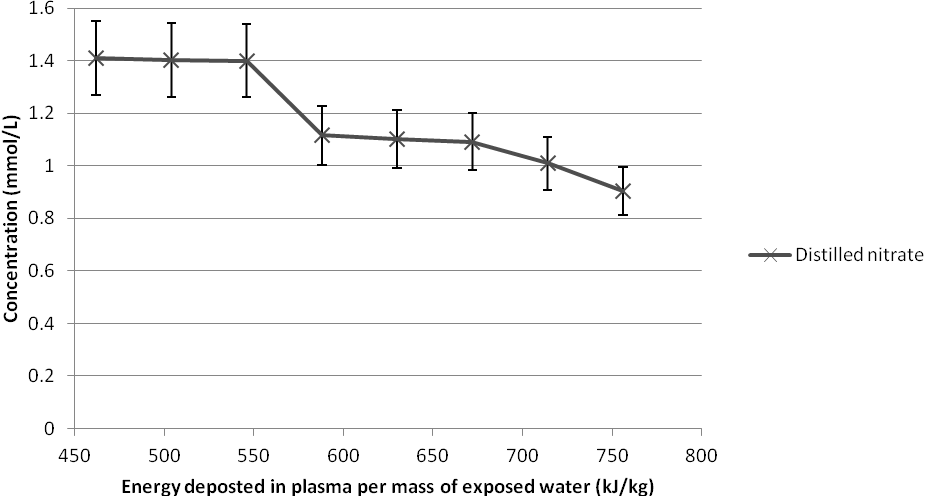
\includegraphics{Figure17_word.png}
  \caption{Nitrate concentration in distilled water versus energy deposited in the plasma per mass of exposed water. No detectable amount of nitrite generated}
  \label{fig:nitrogen_vs_energy}
\end{figure}

\begin{figure}[htbp]
  \centering
  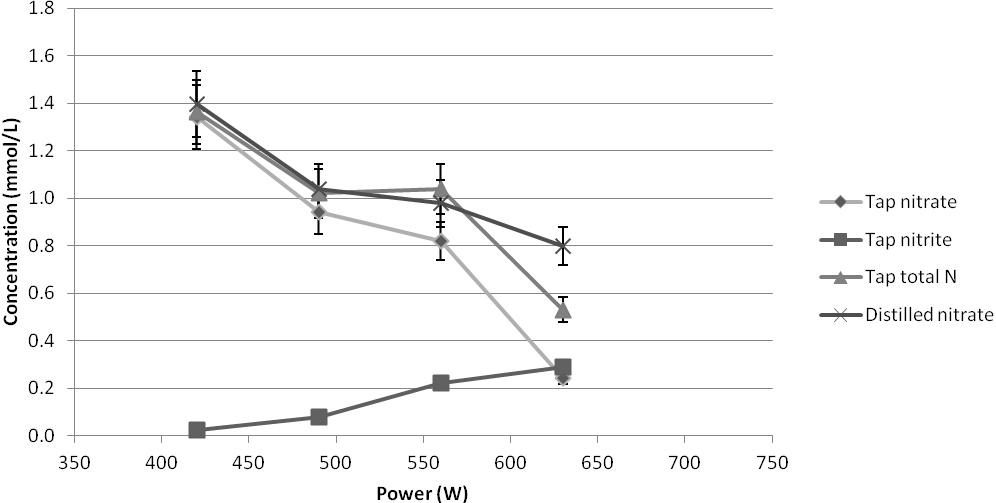
\includegraphics{Figure18_word.png}
  \caption{Nitrate and nitrite concentrations in tap water versus power.  Treatment times scaled such that for each power setting, total energy deposited in system is constant at 504 kJ/kg H2O}
  \label{fig:nitrogen_vs_power}
\end{figure}

Another variable explored was gas flow rate.  For an exposure of 3 minutes, a treatment volume of 150 mL distilled water, and a plasma power input of 420 W, nitrate concentrations were measured for flow rates of .08, .11, and .14 m3/min and are recorded in \cref{fig:nitrogen_vs_flow}.  A factor of 4.9 improvement in nitrate concentration is observed between .08 and .14 m3/min flow settings.  Again no detectable amount of nitrite was observed.

\begin{figure}[htbp]
  \centering
  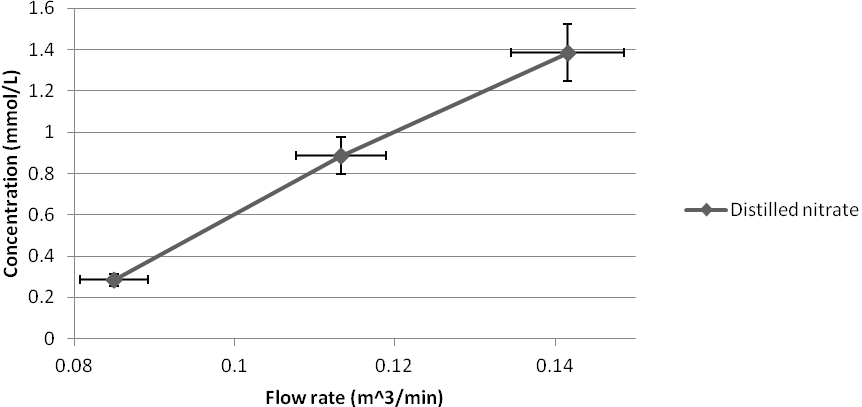
\includegraphics{Figure19_word.png}
  \caption{Nitrate concentration in distilled water versus air flow rate. No detectable amount of nitrite generated}
  \label{fig:nitrogen_vs_flow}
\end{figure}

One variable with remarkable effects on nitrogen species concentration is the presence of basic species before plasma exposure and also addition of basic species after plasma exposure.  As mentioned in the experimental section and as will be touched on further in the discussion section, basic species are known to react with dissolved NO and NO2 (which are formed in the plasma) to form nitrite. \cref{tab:bicarb} summarizes a series of experiments in which the effect of adding approximately 6 mmol/L of sodium bicarbonate before or after plasma exposure was observed on tap and distilled water substrates (200 mL volume).  In both distilled and tap water samples, adding sodium bicarbonate before plasma exposure produced significantly more nitrite than when it was added post-exposure, which in turn produced significantly more nitrite than when no bicarbonate was added at all.  For all three treatment schemes, tap water ended with more nitrite than distilled.  Nitrate trends were not as clear.

\begin{table}[htpb]
  \begin{center}
    \begin{tabularx}{\textwidth}{|c |c |c |X |c |}
      \hline
      \textbf{Nitrite (mmol/L)} & \textbf{Nitrate (mmol/L)} & \textbf{pH} & \textbf{Description} & \textbf{Sample reference \#} \\\hline
      .041 & 1.09 & 3.18 & Tap, no NaHCO3 addition & 1 \\\hline
      2.43 & .795 & 7.99 & Tap, 5.71 mmol/L NaHCO3 added pre-exposure & 2 \\\hline
      .617 & .981 & 7.68 & Tap, 6.19 mmol/L NaHCO3 add post-exposure & 3 \\\hline
      .004 & .795 & 2.88 & Distilled, no NaHCO3 addition & 4 \\\hline
      .854 & .273 & 8.02 & Distilled, 5.71 mmol/L NaHCO3 added pre-exposure & 5 \\\hline
      .235 & 1.37 & 7.55 & Distilled, 6.67 mmol/L NaHCO3 added post-exposure & 6 \\\hline
    \end{tabularx}
  \end{center}
  \caption{Dependence of nitrogen ionic species on water type and amount of NaHCO3 in solution.  The sample \#'s are used as references in the discussion section}
  \label{tab:bicarb}
\end{table}

Another variable that was manipulated was the time between plasma exposure and post-exposure addition of NaHCO3. \Cref{fig:nitrogen_vs_time_delay} shows that while the total molar concentration of ionic nitrogen species is a constant, increasing the time between plasma exposure and NaHCO3 addition increases nitrate concentration and decreases nitrite concentration.

\begin{figure}[htbp]
  \centering
  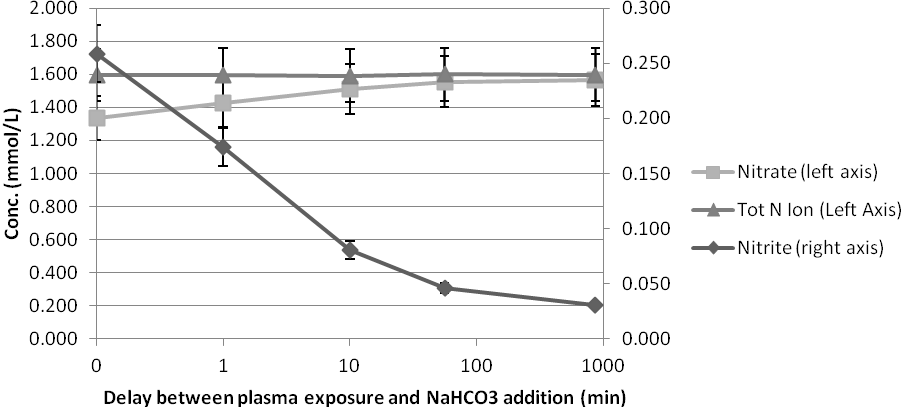
\includegraphics{Figure20_word.png}
  \caption{Effect of time delay between plasma exposure and bicarbonate addition on nitrite and nitrate species concentrations}
  \label{fig:nitrogen_vs_time_delay}
\end{figure}

A fundamental change in the set-up of the system can be realized by removing the stagnant water volume from underneath the electrode and instead spraying the water substrate directly through the active plasma region as described in the experimental section and as shown in \cref{fig:spray_scheme}.  Some difficulty is experienced in maintaining the plasma during water spray operation.  The plasma actively attempts to avoid the region through which the water passes; if the water spray blankets the entire area which the plasma normally occupies, the discharge may extinguish.  However, if the plasma is maintained, the increased biphasic interaction is demonstrated by frequent orange light emission from excited sodium in tap water.  For this alternative geometry the effects of power and gas flow rate on nitrate uptake are in opposition to the trends witnessed for the stationary water phase geometry.   For one pass of distilled water through the active plasma region \cref{fig:nitrogen_vs_energy_spray} shows increasing nitrate uptake with increasing power for a gas flow rate of .11 m3/min (no nitrite formed).  Instead of power on the x-axis, energy per kg of exposed water is used in order to enable a comparison to the results shown in \cref{fig:nitrogen_vs_energy}.  The concentration of nitrate generated in the water is an order of magnitude less in \cref{fig:nitrogen_vs_energy_spray} than it is in \cref{fig:nitrogen_vs_energy}, but the energy usage per kg of exposed water is also an order of magnitude less.  A more obvious comparison between spray and batch treatments can be done by combining \cref{fig:nitrogen_vs_energy,fig:nitrogen_vs_energy_spray} and plotting the amount of nitrate generated per energy usage as a function of power, as is done in \cref{fig:nitro_compare_power}.  The most efficient nitrate generation occurs at 700 W using spray treatment, yielding 4.6 μmols of nitrate per kJ.  However, based on the observed trends, even more efficient nitrate generation may be realized by continuing to increase power with spray treatment or by decreasing power with batch treatment.  \Cref{fig:nitro_vs_flow_spray} shows that spray treatment efficiency may also be improved by decreasing gas flow rate.

\begin{figure}[htbp]
  \centering
  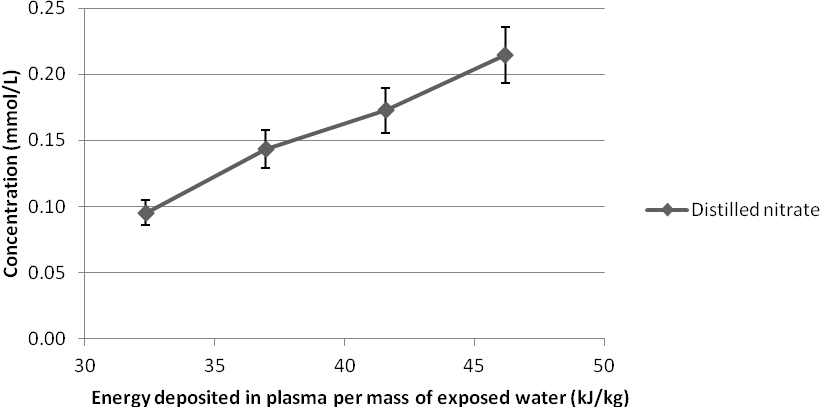
\includegraphics{Figure21_word.png}
  \caption{Dependence of nitrate uptake on plasma energy deposition for water sprayed through the active plasma region.  Compare with results in Figure 17 for batch treatment}
  \label{fig:nitrogen_vs_energy_spray}
\end{figure}

\begin{figure}[htbp]
  \centering
  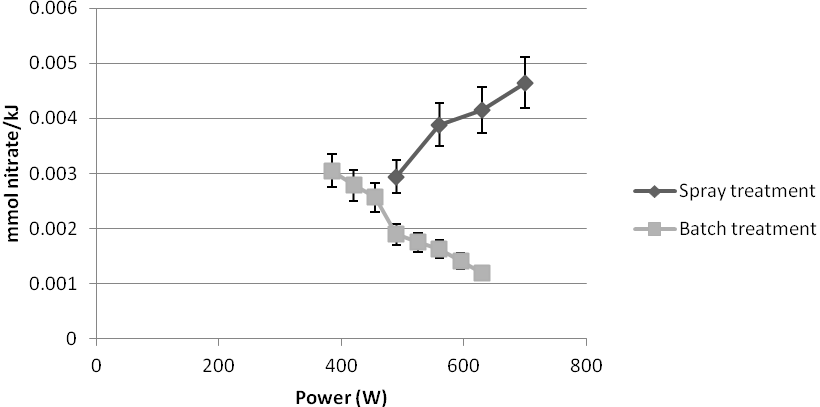
\includegraphics{Figure22_word.png}
  \caption{Comparison between batch and spray treatment methods using mmol of nitrate generated per kJ of electrical energy as the figure of merit.  For lower powers batch treatment is more energetically efficient for nitrate generation.  For higher powers spray treatment is more efficient.  Further investigation of batch process at lower powers and spray process at higher powers required to determine optimal process for nitrate generation}
  \label{fig:nitro_compare_power}
\end{figure}

\begin{figure}[htbp]
  \centering
  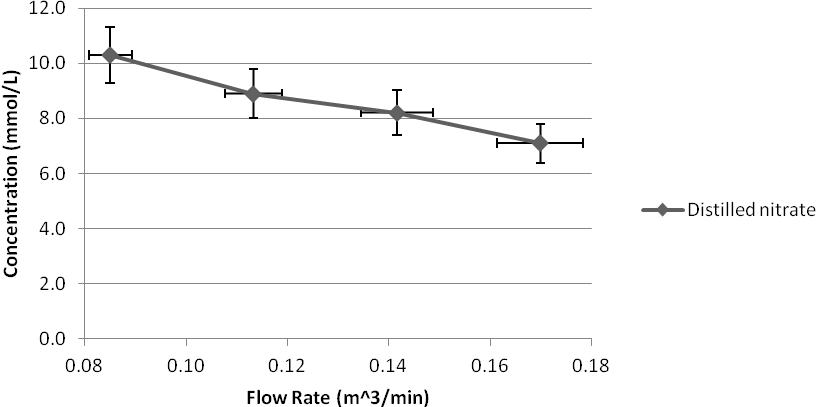
\includegraphics{Figure23_word.png}
  \caption{Dependence of nitrate uptake on gas flow rate for water sprayed through the active plasma region. Power = 560 W.}
  \label{fig:nitro_vs_flow_spray}
\end{figure}

\subsection{Discussion}

\subsubsection{PAW for plant treatment}

Over the course of a four week experiment plants which received PAW in weeks 3 and 4 (CP group) and plants which received PAW for all four weeks (PP group) grew significantly larger than tap water controls (CC group).  Differences between PAW and control groups did not emerge immediately.  As shown in \cref{fig:germ_heights} and by the statistical analysis in \cref{tab:germ_heights_t}, control and plasma treated plants were not significantly different in size after two weeks.  It should also be noted from \cref{fig:germ_sprouts} and \cref{tab:germ_sprouts_t} that PAW and control groups did not show significant differences in germination rates.  However, during the growth phase, weeks 3 and 4, differences between PAW treated plants and tap water controls became evident.  In \cref{fig:radish_span,fig:marigold_span,fig:tomato_span} the increased growth rate of CP and PP plants relative to CC is evident in the sizable slope differences.  The side-to-side photographs in \cref{fig:radish_pic,fig:mari_pic,fig:tomato_pic} show the greater height and foliage of CP and PP plants compared to their CC counterpart.  Moreover, although it is difficult to note in the photographs, CP and PP plants had a healthy, green color at the end of the 4-week experiment; CC plants had begun to yellow and wither.  \Cref{fig:shoots,fig:roots} compare the root and shoot masses for different treatment groups.  \Cref{tab:shoot_t,tab:root_t} show p-values indicating the level of difference in shoot and root masses between groups.  Smaller p-values indicate larger statistical differences; a value of .05 has been chosen as the threshold level to indicate significant statistical differences.  Using that significance level, it is found that CP plants all had significantly larger shoot masses than tap water controls.  PP radishes and tomatoes were significantly larger than controls; PP marigolds were not significantly different from control marigolds (although the p-value of .06 is close to the threshold for significance).  There were not any significant differences between CP and PP shoot masses.  The differences found in shoot masses were not reflected in the root mass data.  \Cref{tab:root_t} shows that no groups demonstrated significant differences in root mass.   The general increase in shoot mass of PAW treated plants is believed to occur primarily because of the nitrate present in PAW after plasma exposure.  Nitrogen is well known to be an essential plant nutrient, necessary for proteins, enzymes, and metabolic processes; ion chromatograph and Total N analyses reveal that nitrite and nitrate are the long-lived nitrogen species in PAW.  Moreover, nitrate concentrations are a factor of 20 larger than nitrite concentrations in these plant experiments and so should be the dominant nitrogen specie that the plants are exposed to.

Error: Reference source not found9] are perhaps the most informative in illustrating the possibility for nitrite to serve as both a fertilizer and an herbicide.    In a control experiment with no sodium nitrite applied to the soil, guinea grass grew to a height of 25 cm.  When sodium nitrite was added such that the soil concentration became 40 ppm, the guinea grass grew to more than double the height of the control, 60 cm.  However, nitrite concentrations above 40 ppm had a less beneficial impact.  An 80 ppm concentration led to a height of 52 cm.  A 120 ppm concentration actually killed 3 of the 6 plant subjects; the average height of the remaining subjects was 44 cm.  It is also important to note that "to avoid killing off seedlings" sodium nitrite was only applied once the grass achieved a height of 12 cm, implying that infant plants are more susceptible to the toxic effects of nitrite accumulation. \cite{zhou2011introduction} It seems reasonable to suggest then that nitrite accumulation in infant plants resulted in the reduced sprout rate observed in the PAW experiment.  It can be theorized that the seedlings absorbed the large amount of nitrate available from PAW, reduced the nitrate to nitrite, and then were unable to rapidly enough convert the nitrite to ammonium, resulting in a toxic accumulation of nitrite.  Once the plants had survived past their infant stages, however, they were capable of more rapidly processing nitrite, eliminating accumulation and allowing them to benefit from the large nitrogen uptake, similar to the effect witnessed in the 40 ppm nitrite sample of [Error: Reference source not found

\subsubsection{Dependence of nitrogen species concentrations on system variables}

The species concentration trends observed in \cref{fig:nitrogen_vs_energy,fig:nitrogen_vs_power,fig:nitrogen_vs_energy_spray} are believed to result from the dependence of electron density and gas temperature on delivered power and from the dependence of interfacial mass transfer on system configuration.   Consider the trend shown in \cref{fig:nitrogen_vs_energy,fig:nitrogen_vs_power} for the concentration of nitrate as a function of power and energy deposition for the case where the water surface is held stationary directly under the plasma.  As power increases, the amount of nitrate produced decreases.  It is possible that the increase in electron density that occurs simultaneously with increasing power creates a more reductive environment which enables more formation of  nitrite as evidenced in \cref{fig:nitrogen_vs_power} (oxidation state = +3) or other more reduced NOx forms such as NO (+2), NO2 (+4), and N2O (+1)  relative to nitrate (+5).  This analysis, however, is confounded by the trend observed in \cref{fig:nitrogen_vs_energy_spray} in which nitrate uptake increases with increasing power when water is sprayed through the active plasma region.  A tentative explanation is that when the water surface is held stationary below the plasma the outgoing convective flow of the feed gas restricts diffusion of water vapor into the plasma region, a restriction that is not present when water is directly injected into the discharge.  If water vapor is present in the active plasma region, an increase in power should correspond to an increase in hydroxyl radical formation because of an increase in the rate of electron-impact dissociation.  This should increase the oxidizing nature of the plasma and subsequently increase nitrate production; this is observed in \cref{fig:nitrogen_vs_energy_spray} for direct water injection.  While this logic may also extend to the case where the plasma hovers over the stationary water surface, it can be expected to occur to a much more limited degree compared to the direct injection case because the convective wind of the feed gas whisks water vapor away from the active plasma region.  Consequently there is not a sufficiently large increase in the oxidizing character of the plasma to offset the increase in reductive character due to electron density; the nitrate concentration then decreases with power as observed in \cref{fig:nitrogen_vs_energy,fig:nitrogen_vs_power}.

The argument presented in the previous paragraph also supports the trend shown in \cref{fig:nitro_vs_flow_spray}, where nitrate concentration decreases with increasing gas flow rate for the case of direct water injection.  An increase in gas flow rate decreases the residence time of gas molecules in the glow region, decreasing the gas temperature.  Decreasing gas temperature decreases the vaporization rate of liquid droplets, leading to a decreased concentration of hydroxyl in the plasma and a decreased ability to oxidize gaseous nitrogen species to nitrate.  This theory, however, contradicts the trend seen in \cref{fig:nitrogen_vs_flow} for stationary water where nitrate increases with flow rate.  One explanation is that the decreased transit time between plasma and water phases results in a decreased radical species recombination rate capable of offsetting the proposed decrease in hydroxyl concentration in the plasma region.

In addition to arguing that increasing hydroxyl concentration in the plasma region should increase the oxidizing nature of the discharge and subsequently increase nitrate concentrations, a stoichiometric outlook suggests that introducing another source of elemental oxygen increases the ratio of oxygen to nitrogen in the discharge, allowing greater formation of high O:N ratio species like NO3-.  This theory will be explored more in future experiments with varying feed ratios of N2 and O2.

In order to address the last variable considered in the study, the effect of basic aqueous species on nitrogen ion concentrations, it is worthwhile to summarize some of the potentially important reaction mechanisms involving reactive nitrogen and oxygen species in solution.   Aside from nitrite and nitrate ions, hydrogen peroxide is known to be a prevailing species in solution following plasma treatment. \cite{traylor2011long}.  Moreover, volatile NOx species like NO and NO2 may also be present and may be responsible for the observation in \cite{traylor2011long} of a spectroscopic peak at 262 nm when samples are sealed; when samples are left unsealed, the 262 nm peak is not observed.  Relevant redox reactions involving these species are taken from \cite{brisset2012peroxynitrite}  and \cite{greenwood1984chemistry} and presented in Table 7.

\begin{table}[htpb]
  \begin{center}
    \begin{tabular}{|l |l |}
      \hline
      \textbf{Reaction Description} & \textbf{Reaction reference \#} \\\hline
      $4NO + O_2 + 2H_2O \rightarrow 4H^+ + 4NO_2^-$ & 1 \\\hline
      $H_2O_2 + NO_2^- \rightarrow ONOO^- + H_2O$ & 2 \\\hline
      $ONOOH \rightarrow H^+ + NO_3^-$ & 3 \\\hline
      $3HNO_2 \rightarrow 2NO + NO_3^- + H^+ + H_2O$ & 4 \\\hline
      $NO + NO_2 + 2A^- + H_2O \rightarrow 2NO_2^- + 2HA$ & 5 \\\hline
      $2NO + O_2 \rightarrow NO_2$ & 6 \\\hline
      $3NO_2 + H_2O \rightarrow 2H^+ + 2NO_3^- + NO$ & 7 \\\hline
      $4NO_2\,(or\,2N_2O_4) + O_2 + 2H_2O \rightarrow 4HNO_3$ & 8 \\\hline
    \end{tabular}
  \end{center}
  \caption{Important reactions between nitrogen and oxygen species which may occur in the aqueous phase}
  \label{tab:reactions}
\end{table}

Reference \cite{greenwood1984chemistry} states that peroxonitrous acid (ONOOH) is formed as an unstable intermediate during the oxidation of acidified aqueous solutions of nitrites to nitrates using H2O2, and that such solutions are more highly oxidizing than either H2O2 or HNO3 alone.  Because the conditions of the former statement are satisfied in PAW, it is reasonable to assume that peroxonitrous acid is the intermediate species between nitrite and nitrate as hypothesized in \cite{traylor2011long}.  Moreover, the much greater efficacy of PAW compared to a control mixture of nitric acid and hydrogen peroxide for degrading bacteria \cite{burlica2010bacteria} further suggests the presence of a reactive oxidizing species like peroxynitrous acid.

Applying the equations in \cref{tab:reactions} to the investigation of basic species effects on nitrogen ion formation provides some insight into observed trends in \cref{fig:nitrogen_vs_time_delay}, where the nitrite and nitrate molar concentrations in PAW as a function of time delay between plasma exposure and addition of sodium bicarbonate are shown.  The +3 oxidation state of nitrogen in water, e.g. nitrite/nitrous acid, is unstable at acidic pH.  Following plasma exposure, PAW is acidic and reaction (4) in \cref{tab:reactions} will occur as long as the solution is acidic.  Subsequently, for long time delays between exposure and base addition, the solution has time to convert nearly all aqueous nitrogen species into nitrate.  If base is added immediately following exposure more nitrite will be preserved in solution.  Moreover, if base is added while +2 and +4 oxidation state nitrogen is present in solution, e.g. species such as NO and NO2, reaction (5) may occur.  It is conceivable that reaction (5) is responsible for the nitrite trends witnessed in \cref{tab:bicarb}.  Tap water contains more basic species than distilled water which theoretically contains none other than a 10-7 molar concentration of hydroxide.  Subsequently, tap water contains more A- species that are capable of reacting with NO and NO2 to form nitrite.  Moreover, if a large quantity of additional base is added to solution before plasma exposure, the amount of A- available for reaction (5) increases significantly, leading perhaps to the comparatively large concentration of nitrite observed in sample 2 in Table 6.  This result is not observed to the same degree in the distilled water sample, sample 5, but some effect is still present.  Relative to solutions that received no additions, the increased presence of nitrite following post-treatment basic additions could be a combination of both reaction (4) and (5) effects, with (5) occurring when base is added quickly enough that NO and NO2 are still dissolved in solution.

Much of the theory suggested above needs to be validated by further experiment and ideally by computational models.  Models should include the relevant chemical reactions shown in \cite{moussa2005acidity}, \cite{brisset2012peroxynitrite}, and \cite{greenwood1984chemistry}.  Rates of primary reactions involving electron-impact ionization, excitation, and bond cleavage will require knowledge of the electron temperature and number density, which are functions of the plasma particle and energy balance.  These balances are derived for low-pressure plasmas in Lieberman \cite{lieberman2005principles} but the highly collisional nature of atmospheric plasmas renders most of the formulas ineffective at high pressures.

\subsection{Summary}

Generating nitrates in water via an atmospheric pressure plasma source shows potential as a process for generating fertilizer.  Plants with shoot masses 1.7-2.2 times larger than tap water treated controls have been grown with PAW.  Subsequent research has focused on increasing the energetic efficiency of generating fertilizing nitrogen species in PAW.  The effects of changing plasma power, gas flow rate, water composition, and system geometry have been investigated.  Varying power and gas flow rate have different effects on NOx (nitrate and nitrite) generation depending on how the water is exposed to the plasma.  For a batch style set-up where the plasma is pointed into a water-containing vessel, increasing plasma power decreases total NOx concentrations and increasing gas flow increases total NOx concentrations.  However, when the water is sprayed sideways through the active discharge region, the opposite power and gas flow trends are observed.  At present the most energetically efficient means of generating NOx is using a 700 W spray treatment, however, observed trends indicate that efficiency may be improved by continuing to increase power with the spray treatment or by exploring low power batch treatments.   Additionally, total NOx concentrations can be dramatically increased by adding basic species to the water before plasma exposure.  It is hypothesized that this increase occurs because of basic species reacting with dissolved NO and NO2 to form nitrite.  In addition to increasing total NOx generation, the addition of bases shifts the solution nitrogen chemistry from nitrate dominated towards higher nitrite content.  For the plant growth experiment conducted in this study, distilled water with no pre-addition of bases was used; thus plants were exposed predominantly to nitrates.  For future fertilizer studies, the effect of nitrite on plant growth must be investigated.

\section{Remediation of Aqueous Pollutants}

As discussed in \cref{chap:intro}, plasmas in contact with liquids produce a cornucopia of reactive species, including both highly oxidative species like OH and highly reductive species like e$^-$. There is considerable interest in the low-temperature plasma community in using these highly reactive species to degrade persistent chemicals in waste streams, both gaseous and liquid. Below, we explore using the VHF atmospheric source to degrade dioxane, a known carcinogen, and perfluorooctanesulfonic acid (PFOS) which has been associated with increased risk of chronic kidney disease. \cite{shankar2011perfluoroalkyl}

\subsection{Dioxane}
\label{sec:dioxane}

In experiment to test the efficacy of plasma for treating dioxane, a 500 mL solution of 400 $\mu$g/L dioxane was treated for 26 minutes with a 420 W air discharge using the geometric configuration shown in \cref{fig:batch_scheme}. The time profile of dioxane concentration is shown in \cref{fig:diox_compare_argon_air}; it follows a simple exponential decay shape. After 26 minutes, 98\% of the dioxane has been removed. This comares very favorably to an AOT study in the literature (\cite{suh2004study}). In the literature study, the treated solution was a factor of two larger; however, the concentration of dioxane was two to three orders of magnitude higher. The plasma decadal treatment time was shorter than the literature study's.

\begin{figure}[htbp]
  \centering
  \includegraphics{air_plasma_treating_dioxane.png}
  \caption{Photograph of 420 W ``calm'' air discharge treating aqueous dioxane solution.}
  \label{fig:diox_air}
\end{figure}

\begin{figure}[htbp]
  \centering
  \includegraphics[width=0.9\textwidth]{argon_plasma_treating_dioxane.png}
  \caption{Photograph of 350 W ``bright'' argon discharge treating aqueous dioxane solution}
  \label{fig:diox_argon}
\end{figure}

A 350 W argon discharge was also used in a dioxane treatment study. Even at a lower power relative to the air discharge, no dioxane was detected after 5 minutes of treatment. This result can be seen in \cref{fig:diox_compare_argon_air}. The almost order of magnitude better performance of argon over air discharge is interesting. Some feeling of the fundamental difference in performance can be gleaned by looking at the appearance of the discharges. The calm air discharge can be seen in \cref{fig:diox_air}; the much brighter and much larger surface area argon discharge can be seen in \cref{fig:diox_argon}. The bright blue color in the argon discharge is likely due to plasma interactions with the aluminum electrode. It is conceivable that the plasma-metal interactions create a larger density of electrons in the discharge that in turn lead to greater creation of oxidative species like OH from water vapor and/or the ambient air. Or it is possible that the greater density in gas phase electrons translates into a greater density of hydrated electrons and that degradation of dioxane may proceed through a reductive pathway as opposed to an oxidative one. Such uncertainty in reaction mechanisms is one of the fundamental reasons that the modelling work described in \cref{chap:basic_science} was begun; until experimental diagnostics are developed that are capable of detailed and comprehensive probing of both gas and near-inteface liquid chemistry, models are a good way to qualitatively explore the plasma-liquid dynamics.

Despite its rapid success in treating dioxane, there are several drawbacks to using the argon discharge. One is that argon is much more expensive than air; for treatment plant wastewater scales, the cost is likely to be prohibitive. Another problem is the erosion of the metal electrode; this could be alleviated by using the pure water electrode configruation (see \cref{fig:water_electrode_scheme,fig:water_electrodes_image}. However, removal of the argon-metal interaction could very well decrase the efficacy of the argon-dioxane treatment. A final problem with argon discharge is its transient nature. When operating the argon discharge, the load impedance can oscillate wildly. This makes impedance matching very difficult, leading to lots of reflected power to the generator. Despite these issues, the argon treatment result is intriguing because of its considerably greater efficacy when compared to leading AOTs like H$_2$O$_2$/O$_3$. Moreover, the air-dioxane treatment, which lacks the issues associated with the argon treatment, also compares reasonably well to the H$_2$O$_2$/O$_3$ method. Finally, as illustrated by the PFOS results presented in \cref{sec:PFOS}, the \cref{fig:batch_scheme} configuration is unlikely to be the best scheme for maximizing plasma-liquid interactions and destroying persistent chemicals. The configuration presented in \cref{fig:water_electrode_scheme} is likely a better choice; indeed a preliminary experiment showed a one-pass reduction in the concentration of dioxane from 365 $\mu$g/L to 172 $\mu$g/L using the pure water electrode design.

\begin{figure}[htbp]
  \centering
  \includegraphics{argon_vs_air_dioxane.png}
  \caption{Comparison of argon and air discharges for removing dioxane from solution}
  \label{fig:diox_compare_argon_air}
\end{figure}

\subsection{PFOS}
\label{sec:PFOS}

 Indeed, when PFOS solution was treated using the geometric configuration shown in \cref{fig:batch_scheme}, no degradation was observed.  However, when PFOS solution was treated using the pure water electrode geometry of \cref{fig:water_electrode_scheme}, degradation was observed. Experimental conditions were 700 W delivered to the plasma, 3 standard cubic meet per minute of air flow, and a roughly 50 $\mu$g/L starting concentration of PFOS. PFOS concentrations were measured using a high performance liquid chromatography (HPLC) instrument provided by the Environmental Protection Agency. The time vs. PFOS concentration profile is shown in \cref{fig:PFOS_degradation}. The curve shows an exponential decay shape that appears to level around a concentration of 5 $\mu$g/L. Ninety percent reduction in PFOS concentration was considered a significant success by colleagues at the EPA. Additional work has focused on trying to elucidate the PFOS degradation mechanism by examining degradation products; however, measurements with HPLC/TOF-MS, ion chromatography, and other methods have been inconclusive. Thus, it is unknown whether PFOS breaks down via oxidative or reductive routes. That the batch treatment scheme was totally unsuccessful in achieving degradation suggests a reductive route since the OH radical concentrations are not expected to vary significantly between \cref{fig:batch_scheme} and \cref{fig:water_electrode_scheme} while the charged particle fluxes, including electrons, are expected to be much larger in the latter case. However, new experimental techniques or detailed models will be required to confirm that hypothesis. This is again motivation for the work that is started in \cref{chap:basic_science}.

\begin{figure}[htbp]
  \centering
  \includegraphics[width=0.9\textwidth]{PFOS_degradation.png}
  \caption{PFOS concentration vs. treatment time using the water electrode}
  \label{fig:PFOS_degradation}
\end{figure}
